\documentclass[a4paper, 12pt]{article}
\usepackage[english]{babel}
\usepackage[utf8]{inputenc}
\usepackage[T1]{fontenc}
\usepackage{lmodern}
\usepackage{hyperref}
\usepackage[numbers, sort&compress]{natbib}
\usepackage{calc}
\usepackage{fancyhdr}
\usepackage{graphics}
\usepackage{nowidow}
\usepackage{color}
\usepackage{subcaption}
\usepackage{epsfig}
\usepackage{epstopdf}
\usepackage{verbatim}
\usepackage{enumitem}


\newlength{\oneLine}
\setlength{\oneLine}{12pt}

\newlength{\eqMargin}
\newlength{\eqHorizMargin}
\newlength{\eqVertMargin}

\setlength{\eqMargin}{20mm}
\setlength{\eqHorizMargin}{\eqMargin}
\setlength{\eqVertMargin}{\eqMargin}

% Paper
\setlength{\paperwidth}{210mm}
\setlength{\paperheight}{297mm}

% Rid the extra space
\setlength{\hoffset}{-1in}
\setlength{\voffset}{-1in}
\addtolength{\hoffset}{\eqHorizMargin}
\addtolength{\voffset}{\eqVertMargin}

% Set margin from the page border (horizontal)
\setlength{\oddsidemargin}{0pt}
\setlength{\evensidemargin}{0pt}

% Header
\setlength{\topmargin}{0pt}
\setlength{\headheight}{42pt}
\setlength{\headsep}{18pt}
\renewcommand{\headrulewidth}{0pt}

% Footer
\addtolength{\footskip}{18pt}
\renewcommand{\footrulewidth}{0pt}

% Margin notes
\setlength{\marginparsep}{0pt}
\setlength{\marginparwidth}{0pt}

% Text
\setlength{\textwidth}{\paperwidth - \hoffset - \hoffset - 25.4mm - 25.4mm}
\setlength{\textheight}{\paperheight - \voffset - \topmargin - \headheight - \headsep - \footskip - \voffset - 25.4mm - 25.4mm}

%\setlength{\labelwidth}{20mm}

% Hyperref settings
\hypersetup{
    unicode=true,					% non-Latin characters in Acrobat's bookmarks
    pdftoolbar=true,				% show Acrobat's toolbar?
    pdfmenubar=true,				% show Acrobat's menu?
    pdffitwindow=false,				% window fit to page when opened
    pdfstartview={FitH},			% fits the width of the page to the window
    pdftitle={S-26.3120 Radio Engineering, laboratory course},	% title
    pdfauthor={Tuomas Leinonen} {Francisco Solano Eizaguirre} {Mikko Heino},	% author
    pdfsubject={Radio Engineering},	% subject of the document
    pdfcreator={LaTeX},				% creator of the document
    pdfproducer={Aalto},			% producer of the document
    pdfkeywords={radio} {antenna} {measurement},	% list of keywords
    pdfnewwindow=true,				% links in new window
    colorlinks=true,				% false: boxed links; true: colored links
    linkcolor=black,				% color of internal links
    citecolor=black,				% color of links to bibliography
    filecolor=black,				% color of file links
    urlcolor=black					% color of external links
}

% Bad hyphenation
%\hyphenation{}

\newcommand{\dB}{\ensuremath{\mathrm{dB}}}

\definecolor{dkred}{rgb}{0.6, 0, 0}
\definecolor{dkgrn}{rgb}{0, 0.6, 0}
\definecolor{dkblue}{rgb}{0, 0, 0.6}

\newcommand*{\mysection}[1]{%
\newpage%
\section*{#1}%
\addcontentsline{toc}{section}{#1}%
}

\pagestyle{fancy}
\lhead{S-26.3120 Radio Engineering, laboratory course\\Lab 3: Antenna Measurements -- Final Report\\}
\rhead{Tuomas Leinonen, 84695P\\Francisco Solano Eizaguirre, 401049\\Mikko Heino, 79657L}
\cfoot{\thepage}


\begin{document}

\begin{titlepage}
\pagestyle{empty}
\begin{center}

\vspace*{30mm}
\noindent\LARGE{\textbf{S-26.3120 Radio Engineering, laboratory course}}

\vspace*{20mm}

\Large{\textbf{Lab 4: Amplifier}}\\

\vspace*{15mm}

\large{\textbf{Final Report}}\\
\vspace{15mm}
\large{\today}
	
\vspace*{30mm}
\large{
	\begin{tabular}{l l}
		\textbf{Group 1:} 				& \\
		Tuomas Leinonen 				& 12345A \\
		Gaurav							& 12345A \\
		Jalmari							& 12345A
	\end{tabular}
}

\end{center}

\end{titlepage}

\mysection{Abstract}

Text

\newpage
\addcontentsline{toc}{section}{Contents}
\tableofcontents

\mysection{Symbols and abbreviations}

\subsection*{Symbols}

	\begin{description}[font=\rmfamily\mdseries, leftmargin=25.5mm, style=sameline, align=right, labelsep=5mm, itemsep=-2pt]
		\item[$C$]					kapasitanssi
		\item[$f$] 					taajuus
		\item[$Z$] 					impedanssi
	\end{description}

\subsection*{Abbreviations}

	\begin{description}[font=\rmfamily\mdseries, leftmargin=25.5mm, style=sameline, align=right, labelsep=5mm, itemsep=-2pt]
		\item[LOL]					lots of love
	\end{description}

\newpage
\section{Introduction}

Test

\begin{figure}[h!]
	\begin{center}
	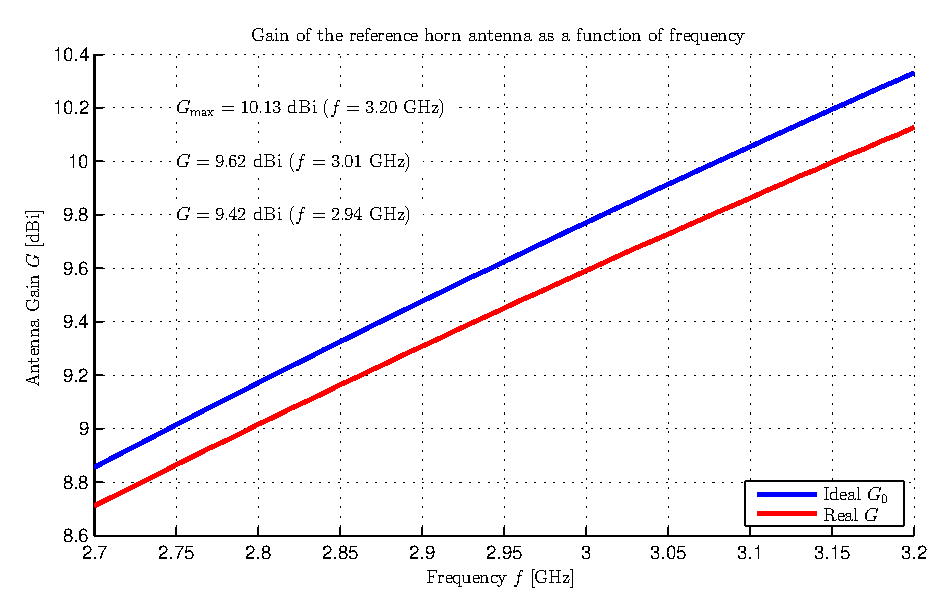
\epsfig{width=0.8\textwidth, file=img/horn.eps}
	\caption{Example figure.}
	\label{f:horn}
	\end{center}
	\vspace*{-\oneLine}
\end{figure}

\begin{equation}\label{e:F}
F = ma
\end{equation}


\newpage
\section{Conclusions}

Text

\newpage
\section{Feedback}

Text


\newpage
\begin{thebibliography}{9}%\itemsep 7pt\parskip -5pt 

\bibitem{mikro} A.\ Lehto, A.\ Räisänen, 
	\textit{Mikroaaltomittaustekniikka}, Otatieto, 1991.
	
\bibitem{parts} M.\ Steer, 
	\textit{Microwave and RF Design -- A Systems Approach}, 
	SciTech Publishing, 2010. 
	ISBN: 978-1-891-12188-3.
	
\bibitem{lsh} C.\ Icheln (edited), 
	\textit{Lecture supplement handout},
	S-26.3120 Laboratory course in Radio Engineering course material.
	
%\bibitem{lab3} C.\ Icheln, 
%	\textit{Instructions for Lab III: Antenna Measurements},
%	S-26.3120 Laboratory course in Radio Engineering course material.
	
%\bibitem{slides} C.\ Icheln, 
%	\textit{Lecture slides},
%	S-26.3120 Laboratory course in Radio Engineering course material.

%\bibitem{pozar} D.\ M.\ Pozar, 
%	\textit{Microwave Engineering}, 
%	J.\ Wiley \& Sons, 4th Ed., 2012. 
%	ISBN: 978-0-470-63155-3.
	
%\bibitem{gains} J.\ C.\ Logan, J.\ W.\ Rockway, 
%	``Dipole and Monopole Antenna Gain and Effective Area for Communication Formulas.''
%	Available online at \url{www.dtic.mil/cgi-bin/GetTRDoc?AD=ADA332891}
%	[Retrieved: November 25th, 2013].

%\bibitem{parts} M.\ Steer, 
%	\textit{Microwave and RF Design -- A Systems Approach}, 
%	SciTech Publishing, 2010. 
%	ISBN: 978-1-891-12188-3.
	
%\bibitem{kandi} T.\ Leinonen, 
% 	``Antenna and front-end challenges for mobile software-defined radio receiver,''
%	B.\ Sc.\ (Tech.) thesis (in Finnish), 2012. 
% 	Available online at \url{http://urn.fi/URN:NBN:fi:aalto-201301161154}.
	
%\bibitem{iet} R.\ J.\ Collier, A.\ D.\ Skinner (editors), 
%	\textit{Microwave Measurements}, 
%	The Institution of Engineering and Technology, 3rd Ed., 2007. 
% 	ISBN: 978-0-86341-735-1.

\end{thebibliography}

\end{document}
